
% Complete documentation on the extended LaTeX markup used for Insight
% documentation is available in ``Documenting Insight'', which is part
% of the standard documentation for Insight.  It may be found online
% at:
%
%     http://www.itk.org/

\documentclass{InsightArticle}

\usepackage[dvips]{graphicx}
\usepackage{xspace}
\usepackage{dsfont}
%%%%%%%%%%%%%%%%%%%%%%%%%%%%%%%%%%%%%%%%%%%%%%%%%%%%%%%%%%%%%%%%%%
%
%  hyperref should be the last package to be loaded.
%
%%%%%%%%%%%%%%%%%%%%%%%%%%%%%%%%%%%%%%%%%%%%%%%%%%%%%%%%%%%%%%%%%%
\usepackage[dvips,
bookmarks,
bookmarksopen,
backref,
colorlinks,linkcolor={blue},citecolor={blue},urlcolor={blue},
]{hyperref}


%  This is a template for Papers to the Insight Journal. 
%  It is comparable to a technical report format.

% The title should be descriptive enough for people to be able to find
% the relevant document. 
\title{Statismo - A framework for PCA based statistical models.}

% 
% NOTE: This is the last number of the "handle" URL that 
% The Insight Journal assigns to your paper as part of the
% submission process. Please replace the number "1338" with
% the actual handle number that you get assigned.
%
\newcommand{\IJhandlerIDnumber}{1338}
%\newcommand{\statismo}{\emph{statismo}\xspace}
\newcommand{\Statismo}{\emph{Statismo}\xspace}
\def\R{\mathds{R}} %reelle Zahlen

% Increment the release number whenever significant changes are made.
% The author and/or editor can define 'significant' however they like.
\release{0.80}

% At minimum, give your name and an email address.  You can include a
% snail-mail address if you like.
\author{Marcel L\"uthi$^{1}$, R{\'e}mi Blanc$^{2}$, Thomas Albrecht$^{1}$, Tobias Gass$^{3}$, Orcun Goksel$^3$, Philippe B\"uchler$^{4}$, Michael Kistler$^4$, Habib Bou-Sleiman$^4$,  Mauricio Reyes$^{4}$, Philippe C. Cattin$^{5}$, Thomas Vetter$^{1}$ }

\authoraddress{$^{1}$Department of Mathematics and Computer Science, University of Basel, Switzerland\\
               $^{2}$University of Bordeaux (TODO WHICH INSTITUTE!!!!), France\\
               $^{3}$Computer Vision Lab, ETH Zurich, Switzerland \\
               $^{4}$Institute for Surgical Technology and Biomechanics, University of Berne, Switzerland  \\
               $^{5}$Medical Image Analysis Center, University of Basel, Switzerland 
             }


\begin{document}



%
% Add hyperlink to the web location and license of the paper.
% The argument of this command is the handler identifier given
% by the Insight Journal to this paper.
% 
\IJhandlefooter{\IJhandlerIDnumber}


\ifpdf
\else
   %
   % Commands for including Graphics when using latex
   % 
   \DeclareGraphicsExtensions{.eps,.jpg,.gif,.tiff,.bmp,.png}
   \DeclareGraphicsRule{.jpg}{eps}{.jpg.bb}{`convert #1 eps:-}
   \DeclareGraphicsRule{.gif}{eps}{.gif.bb}{`convert #1 eps:-}
   \DeclareGraphicsRule{.tiff}{eps}{.tiff.bb}{`convert #1 eps:-}
   \DeclareGraphicsRule{.bmp}{eps}{.bmp.bb}{`convert #1 eps:-}
   \DeclareGraphicsRule{.png}{eps}{.png.bb}{`convert #1 eps:-}
\fi


\maketitle


\ifhtml
\chapter*{Front Matter\label{front}}
\fi


% The abstract should be a paragraph or two long, and describe the
% scope of the document.
\begin{abstract}
\noindent
This paper describes the \Statismo framework,  which is a framework for PCA
based statistical models.  Statistical models are used to describe the
variability of an object within a population, learned from a set of
training samples. Originally developed to model shapes, statistical models are now increasingly used to model 
the variation in different kind of data, such as for example images, volumetric meshes or deformation fields. 

\Statismo has been developed with the following main goals in mind:
$1)$ To provide a generic tools for learning all kinds of PCA based
statistical models, such as shape, appearance or deformations models.
$2)$ To make the exchange of PCA models easier among different
research groups and to improve the reproducibility of the models.
$3)$ To allow for an easy integration of new methods for model
building into the framework.  To achieve the first goal, we have
abstracted all the aspects that are specific to a given model and data
representation, into a user defined class. This does not only make it
possible to use \Statismo to create all different kinds of PCA models,
but also allows \Statismo to be used with any toolkit and data format.
To facilitate data exchange, \Statismo defines a storage format based
on HDF5, which includes all the information necessary to use the
model, as well as meta-data about the model creation, which helps to
make model building reproducible.  The last goal is achieved by
providing a clear separation between data management, model building
and model representation.  In addition to the standard method for
building PCA models, \Statismo already includes two recently proposed
algorithms for building conditional models, as well as convenience tools
for facilitating cross-validation studies.

Although \Statismo has been designed to be independent of a particular toolkit, special efforts have been
made to make it directly useful for VTK and ITK. Besides supporting
model building for most data representations used by VTK and ITK, it
also provides an ITK transform class, which allows for the integration
of \Statismo with the ITK registration framework. This leverage the
effort that has been done in ITK, to obtain powerful methods for model
fitting.

\end{abstract}

\IJhandlenote{\IJhandlerIDnumber}

\tableofcontents

\section{Introduction}

Statistical models have become a firmly established tool in computer
vision and medical image analysis.  They model the variability of a
class of objects by means of a multivariate normal distribution,
learned from example data.  In particular in the form of shape models,
they have been employed in a wide range of applications such as object
recognition \cite{cootes_use_1994, paysan_3d_2009}, image manipulation
\cite{blanz_morphable_1999}, surgery planning
\cite{zheng_statistical_2011,hawkes_tissue_2005} or implant design
\cite{bou-sleiman_minimization_2011,kozic_statistical_2009}.
Furthermore, they have been used as a prior for different algorithms,
such as segmentation \cite{heimann_statistical_2009} or registration
\cite{albrecht_statistical_2008}.  In spite of their success, there is
still no established toolkit for the creation and application of such
models. This requires the same method to be implemented over and over
again. Moreover, it makes the exchange of models difficult, and thus
hinders the collaboration between different researchers as well as the
reproducibility of experiments.  In this paper we introduce the
\Statismo framework, which is a \C++ framework for the creation and
use of different kinds of statistical models.  In contrast to other
libraries (such as the statistical models currently implemented in
ITK), \Statismo provides a high-level interface: Statistical models
are interpreted as a probability distribution over the modeled object,
from which samples (i.e.\ shapes, images, etc.)  can be drawn and
probabilities of object instances can be computed.  The current
implementation focuses on the most commonly used type of statistical
models, i.e.\ PCA-based shape models, and its associated statistical
interpretation as a multivariate normal distribution.

The standard example for a statistical PCA model is the statistical
shape model.  It represents a class of shapes in terms of deformations
of a triangulated reference surface. Nevertheless the concept can be
applied to various other types of data, such as images, displacements
fields, volumetric meshes, etc. Independent of the concrete type of
model, the statistical analysis requires each dataset to be converted
in to a vectorial representation.  \Statismo provides a unified
treatment of these models by letting the user provide special template
classes, so called \emph{Representer} classes, which define this
conversion.  Depending on the type of data, this may include
preprocessing steps, such as establishing correspondence or alignment of
the datasets.  A representer also provides the reverse
functionality, to convert the vectorial representation back to its
original representation.  The abstraction introduced by the
Representer does not only allow for a unified treatment of different
kinds of PCA based models, but also to make \Statismo independent of
the library used to represent the data. Thus the exact same code that
is used for creating a shape model from shapes represented in VTK can
also be used for creating deformation models from ITK displacement
fields.

One of the main design goals of \Statismo is to facilitate the
exchange of statistical models among different research groups and end
users. We therefore defined a platform independent storage based on
HDF5 \cite{hdf5}. \Statismo stores all the information needed to
capture the complete probabilistic interpretation of the model.  This
requires in particular that all the pre-processing steps, such as
alignment or normalization can be reproduced. \Statismo enforces this
by requiring the same Representer to be used in the application of the
model, as was used for model building. Moreover, \Statismo stores all
the parameters and additional metadata necessary to make the models
more easily reproducible.  Another goal of \Statismo is to allow for
the easy integration of different model building algorithms. This is
achieved by the modular design of the data management, model building
and model representation components. Thus, new algorithms for model
building can be easily integrated into \Statismo and make use of all
the functionality already implemented.  In addition to standard PCA
models, \Statismo currently supports the building of conditional
models based on surrogate variables \cite{blanc_conditional_2009}, as
well as geometric constraints \cite{luthi_probabilistic_2009}.

\Statismo includes standard Representers for the most commonly used
data representations in VTK and ITK, making it possible to build and
exchange PCA based shape models, image models, and deformation models,
using both ITK and VTK. \Statismo also provides wrapper classes that
allow for the seamless integration of \Statismo into ITK. Furthermore,
a special itkTransform class is provided, which makes it possible 
to exploit the power of the  ITK Registration Framework for
statistical model fitting.


\section{Background: PCA based statistical models}
\subsection{General Introduction}\label{sec:pca-models}
The idea behind PCA Models is to learn a (linear) model for an object class from a set of
typical example of this class. Let $\mathcal{O} = \{O^1, \ldots,
O^n\}$ be a set of training examples. These
objects can for example be images, deformation fields or shapes. Model
building consists of the following three steps:
\paragraph{1) Discretization:} This aims to define a discrete
domain $\Omega = \{p_1, \ldots, p_N\}$ on which we approximate all the objects. I.e.\ we define an object as
\[
\hat{O}^i = (\varphi^i(p_1), \ldots, \varphi^i(p_N)), \; i  = 1 \dots, n. 
\]
For shape models, the domain $\Omega \subset \R^3$ is usually defined
by the points of a 3D reference mesh and $\varphi^i : \R^3 \to \R^3$
is a function that maps each point $p_i$ to the corresponding point of
the target shape $\hat{O}^i$. For images $\Omega$ is an image domain
and $\varphi^i : \Omega \to \R$ that assigns to each point its image
intensity. Similarly, for deformation models $\varphi^i : \Omega \to
\R^d$ assigns to each point a deformation that is defined on the
deformation field $\hat{O}^i$.

Note that this definition implies correspondence between all the examples. The
exact notion of correspondence depends both on the type of objects and the
application. Ensuring the correspondence between the examples is usually done by performing a registration.
\paragraph{2) Normalization:}
Depending on the type of the objects, further preprocessing steps may
follow. Shapes, for example, are usually rigidly aligned using
Procrustes registration before building the model. For images, a
histogram equalization or a low pass filtering may be performed to
reduce the excess variability of the samples.
\paragraph{3) Model building:}
Once the shapes are processed, each object $O^i$ can be
represented as a high-dimensional vector 
\[
v^i = (\varphi^i(p_1), \ldots, \varphi^i(p_N)) \in \R^{N\cdot d}.  
\]
PCA estimates an orthonormal basis spanning this
high-dimensional space, defined iteratively as the directions onto
which the projection of the data has maximum variance. This offers the
opportunity to reduce the dimensionality of the model, keeping only
the principal directions covering a prescribed proportion of the total
data variability.  Mathematically, these are obtained from the sample mean and sample covariance matrix of the 
training data, using the usual formula from statistics:
\begin{equation}
 \begin{split}
   \overline{m} & = \frac{1}{n} \sum_{i=1}^n v_i \\
   S &= \frac{1}{n-1} \sum_{i=1}^n (v_i - \overline{m}) (v_i - \overline{m})^T.
   \end{split}
\end{equation}
Using a singular value decomposition, the sample Covariance Matrix is decomposed
as $S=UD^2V^T$. The column $u_i$ of the 
matrix $U \in \R^{Nd \times {n}}$ is referred to as the $i$-th principal component.
The principal components form a basis for the vector space in which all the examples are defined. 
An entry $\lambda_i$ in the diagonal matrix $D^2 = \text{diag}(\lambda_1, \ldots, \lambda_{n})$,  denotes how much variance is represented by the $i$-th principal component \cite{mardia_multivariate_1980}.
A statistical model is defined as the low dimensional generative model, that
\[
v = v(\alpha_1, \ldots, \alpha_m) = \overline{m}  + \sum_{i=1}^m \alpha_i \lambda_i u_i, 
\]
where $m < n$ is the number of principal components that are used to model span the model. 
Each vector $\alpha = (\alpha_1, \ldots, \alpha_m)$ introduces a unique shape. 
Usually it is assumed that $\alpha$ follows a standard normal distribution: 
\begin{equation} \label{eq:coeff-normal-assumption}
\alpha  \sim \mathcal{N}(0, I_m)
\end{equation}
This in turn introduces a probability distribution over the discretized vectors representing the objects, namely 
\begin{equation} \label{eq:prob-interpretation}
v \sim \mathcal{N}(\overline{m}, UD^2U^T) \approx \mathcal{N}(\overline{m}, S).
\end{equation}

% The simplest use of a statistical model is to visualize the variability
% of an object class by drawing samples from the distribution it
% represents.  Another main application is to use the model as a prior
% over the possible objects, such as a shape prior in segmentation.
% Also, it can be used in inference, to reconstruct an unobserved part
% of an object (such as e.g.\ a trauma) in a probabilistically sound
% way.  It is important to note that to correctly use this probabilistic
% model \eqref{eq:prob-interpretation} for a new object, the object
% needs to be represented and normalized in exactly the same way as the
% training examples $O_1, \ldots, O_n$.

\subsection{Probabilistic PCA}
In section \ref{sec:pca-models} we have sketched the basic idea behind
PCA based statistical models, as it is commonly presented and used in the
literature.  There is, however, a flaw with this simple probabilistic
interpretation (Cf. Equations \eqref{eq:coeff-normal-assumption} and
\eqref{eq:prob-interpretation}).  This model assumes that all the
probability mass is concentrated on the subspace spanned by the
principal components.  Thus the probability of an object that does
not strictly lie in this subspace is zero. In practice, however, an object might be a valid and likely instance of the class and 
still not lie exactly on that subspace. This may on one hand happen since this subspace is only approximated from a finite number of examples, 
but also because the data itself is usually noisy.
% To see why this is a
% problem, assume that we have left out one of the $n$ example shapes and
% build the shape model from the remaining $n-1$ examples. Because the
% left out example is from the same class as the other shapes, it will
% be very close to the span of the remaining shapes. However, it will in
% general not lie exactly \emph{in} the span. Thus the probability of
% this example becomes zero, although we know that it is in fact a member
% of the object class represented by the model. 
 To alleviate this
problem, Probabilistic PCA (PPCA) \cite{tipping_probabilistic_1999} is used in \Statismo.
PPCA  provides a well defined probabilistic interpretation, by assuming
a small amount of noise on the examples. The new generative
model is of the form
\[
v = v(\alpha_1, \ldots, \alpha_n) = \mu  + \sum_{i=1}^n \alpha_i \lambda_i u_i + \varepsilon
\]
with $\varepsilon \sim \mathcal{N}(0, \sigma^2)$.  By virtue of the
added noise term, this model now defines a valid probability distribution
on the whole of $\R^{Nd}$. The probability for instances now depends
on the distance from this subspace. Objects that are far away are less
likely than those instances that are close to the space.  It can be
shown that when $\sigma^2$ goes to $0$ a standard PCA model is
obtained \cite{roweis_em_1998}.

\section{Design / Architecture}
\Statismo has been designed to achieve the following goals:
\begin{description}
\item[High level:] Most applications of statistical model exploit the
  fact that statistical models define a probability distribution of
  the modeled objects. The interface of \Statismo is designed to reflect this fact and provides
  high-level methods to work with the represented distribution, rather than 
  exposing the eigenvalues and eigenvectors of the model. 
\item[Independence of data representation:] 
  Statistical models are used to model the variation in various types of objects, using a variety of 
  different toolkits to represent the data. Independently of the concrete representation of the data, 
  the ideas and interpretation of PCA-based  statistical models is always the same. 
  \Statismo is designed to work for any kind of PCA models, independently of the data representation or the toolkit used. 
\item[Reproducibility and easy data exchange:] 
  It is often fruitful to exchange statistical models with colleagues or other researchers. 
  An important design goal is to facilitate this exchange by providing a platform independent data format, 
  which contain all the information needed to use the model from an application. 
  Furthermore, to help reproduce an experiment the stored model should contain all the parameters
  that were used to build the model. 
\item[Flexibility and Extensibility:] 
  \Statismo should make it easy to integrate new algorithm for model building. 
  This will on one hand increase the usefulness of \Statismo itself, but also 
  allow the algorithms to benefit from the facilities implemented in \Statismo. 
\end{description}


\subsection{Design overview}\label{sec:design-overview}
To ensure flexibility and  extensibility, \Statismo uses a modular structure that clearly separate 
data management, model building and model representation. 
Figure~\ref{fig:class-diagram} shows a class diagram of \Statismo.
\begin{figure}
  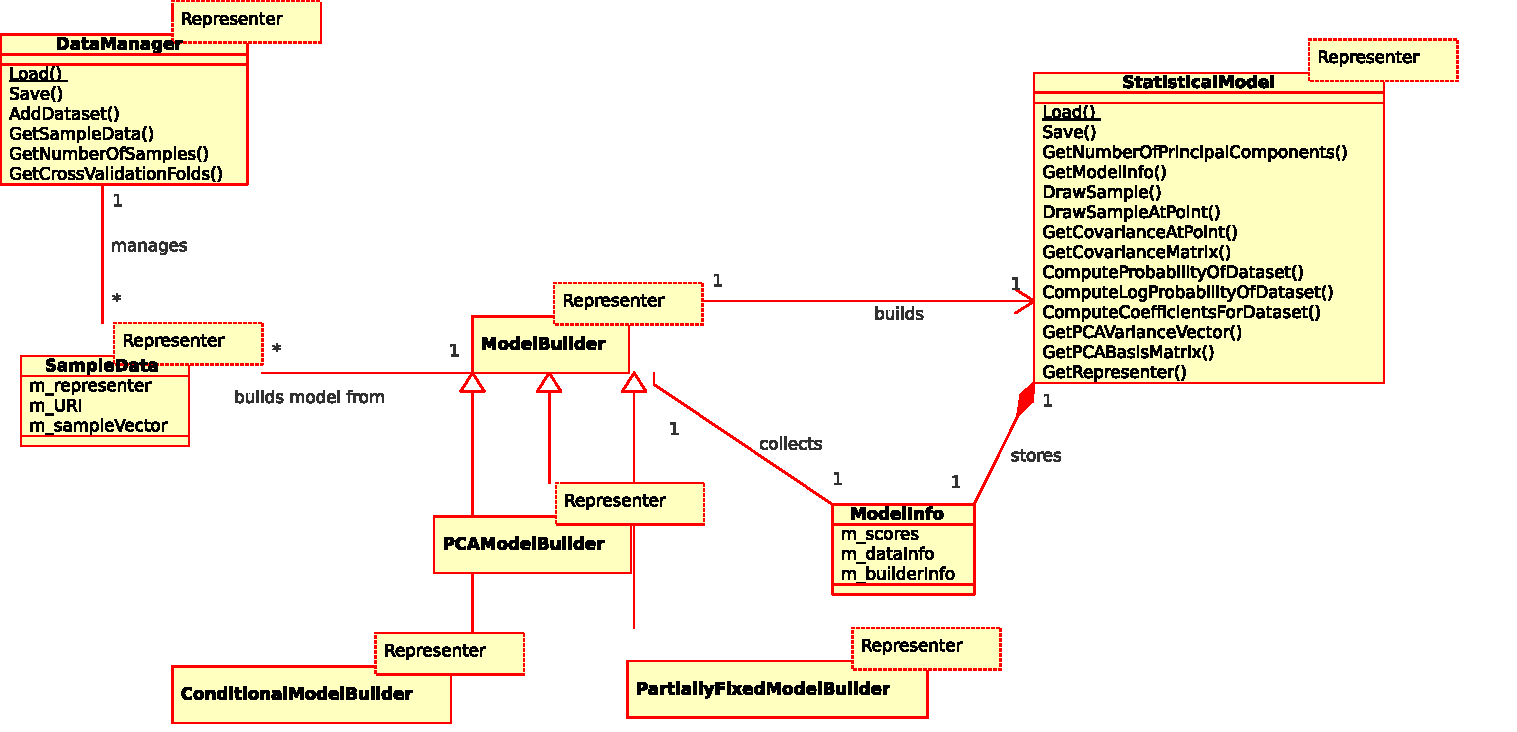
\includegraphics[width=\textwidth]{pictures/class_diagram.pdf}
  \itkcaption{The core classes in \Statismo}
  \label{fig:class-diagram}
\end{figure}
The data used to build the model is added to the data manager
\code{DataManager} class, via the \code{AddDataset} method. This
method first preprocesses (e.g.\ aligns and normalizes) the dataset
and converts it into an internal vectorial representation, which is
stored together with metadata, such as the URI of the dataset. These
preprocessed datasets are referred to as \emph{samples}. The
\code{ModelBuilder} class takes a list of samples and uses it to build
a statistical model. The \code{ModelBuilder} class is also responsible
for collecting all the metadata associated with the samples, which are then
stored together with additional information set by the model builder (such as
the build time, parameter settings, etc.) in the \code{ModelInfo}
class. The \code{StatisticalModel} class resulting from the
\code{ModelBuilder} can now be used independently of the other
classes. It contains all the information needed in the application of
a statistical model and accordingly is saved in a platform independent storage format 
based on HDF5. 

\subsubsection{A note on the terminology}
Most terminology used in \Statismo is directly motivated by the
probabilistic interpretation, and does not require further
clarification.  However, while in statistics the term \emph{sample} and
\emph{dataset} are usually used synonymously, in \Statismo these terms have precise
meanings.  An \emph{dataset} is a representation of an object used as an input to build the model.  A \emph{sample}
represents the same object but after discretization and normalization have been applied
to it (Cf. Section~\ref{sec:pca-models}).  It is an instance of the
object as it is represented by the model.  The probability distribution defined by the statistical model, 
models the probability of the \emph{samples} but not of the \emph{datasets}. 
Finally, a \emph{sample
 vector} is the representation of a \emph{sample} as a vector. 


\subsection{Representers} \label{sec:representers} 
The key concept that allows \Statismo to be independent of a specific data representation, and to build all types of PCA models is the concept of a \emph{Representer}. Every class in \Statismo is parametrized over a user-defined \code{Representer} class. 
A \code{Representer} class has two distinct purposes: First, it is used
as an adapter class to convert between the data representations used
by an application and the internal representation used by
\Statismo. This allows \Statismo to be used with a variety of
different toolkits. Second, it also defines how the objects are
processed before they are used for building the model.  Recall from
Section~\ref{sec:pca-models} that before a model is built, objects are
discretized, normalized and converted into a consistent vectorial
form.  The discretization and normalization step are specific to the
type of object that are modeled.  A \code{Representer} class in
\Statismo needs to provide the methods
\code{Representer::DatasetToSample},
\code{Representer::SampleToSampleVector} and
\code{Representer::SampleVectorToSample}.  The first method takes care
of the discretization and normalization, the second method is used to
convert a dataset to its vectorial representation.  The last method is
used to convert the vectorial representation back to an object of the
modeled type. Figure~\ref{fig:statismo-flow} illustrates this concept.
The input to \Statismo is always a dataset. This is converted into a
sample, and then in its vectorial representation, from which all the
statistics is computed.  Note that the vectorial representation is
never exposed to the user, but it is always converted back to the
sample representation. For shape models, for instance, the output
sample is a mesh, in the specific data representation used by the \code{Representer}.
\begin{figure}
  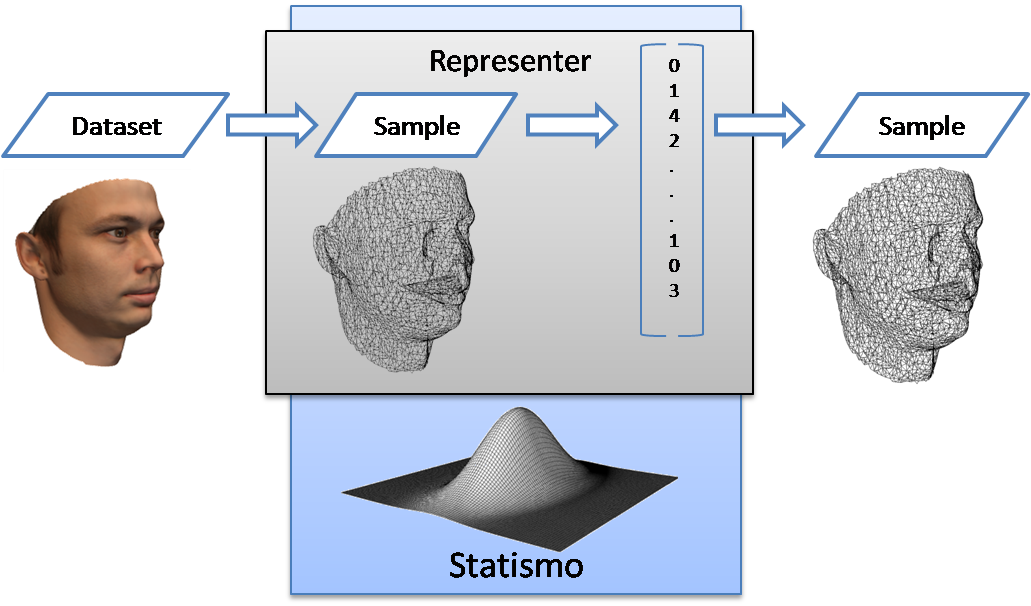
\includegraphics[width=\textwidth]{pictures/statismo_flow.png}
  \itkcaption{The dataflow in \Statismo.  Inputs to \Statismo are datasets, in a user defined data representation. 
    The output is always a sample from the probability distribution over the objects that are modeled. }
    \label{fig:statismo-flow}
\end{figure}


\subsection{ITK Support}
\Statismo was designed to work together with many different toolkit
and libraries. It was therefore not possible to follow
library-specific conventions. \Statismo therefore has its own
conventions. These were chosen to make as few assumptions as possible
for the user. For example, no smart pointer is used in \Statismo, as
this would restrict the user to use the same smart pointer when using
\Statismo. Using the generic \Statismo interface, a code snippet to
load a model looks like
\begin{verbatim}
statismo::StatisticalModel<RepresenterType>* model = 
    statismo::StatisticalModel<RepresenterType>::Load("model.h5");
SampleType* sample = model->DrawSample();
delete model;
\end{verbatim}
Nevertheless, ITK being a major focus of \Statismo, we
provide special wrappers that follow the ITK conventions and provide a seamless integration of  \Statismo in ITK. 
Accordingly, the same code snippet will look like
\begin{verbatim}
itk::StatisticalModel<RepresenterType>::Pointer model = 
    itk::StatisticalModel<RepresenterType>::New();
model->Load("model.h5");
SampleType::Pointer sample = model->DrawSample();
\end{verbatim}
The main difference between the two interfaces, is that the former generic \Statismo interface
requires all arguments as the object is created
(here with the Load function) and thus ensures that 
the objects themselves are well defined after construction.
The memory management is done manually whereas, with the ITK Wrapper, the memory is managed using the ITK smart pointers. 

Specifically for ITK, \Statismo also provides a class \code{itk::StatisticalModelTransform}, which 
enables the use of statistical models as ITK transforms. This has great practical value since these transform can then be used in the  ITK registration framework for statisitical model fitting. 


\section{Using \Statismo}
In this section we illustrate how \Statismo can be used to perform typical tasks related with statistical models:
\begin{enumerate}
  \item Generation and storage of a statistical model
  \item Loading a model from disk
  \item Visualizing the variability in  a model
  \item computing the likelihood of a dataset
  \item performing a cross-validation experiment
  \item using the ITK registration framework for model fitting. 
\end{enumerate}
Most examples below use  the generic
interface with the \code{vtkPolyDataRepresenter}. This representer is
created by providing it with a reference dataset that defines the
discretization and mesh topology. Before converting a dataset to its
vectorial representation, it performs a Procrustes alignment
\cite{horn_closed-form_1987} of the dataset to the reference, and thus normalizes pose
variations automatically. Note that this representer assumes, that the
datasets are already in correspondence.

The last example illustrates the use of \Statismo with the ITK
registration framework and makes use of the ITK Wrappers for
statismo. For this we use the \code{itkMeshRepresenter} that represents datasets
of type \code{itk::Mesh}. 


\subsection{Building statistical models in \Statismo}

The first step in using \Statismo is to define which representer is used and to parametrize all classes with that 
representer. 
\begin{verbatim}
  typedef vtkPolyDataRepresenter RepresenterType;
  typedef PCAModelBuilder<RepresenterType> ModelBuilderType;
  typedef StatisticalModel<RepresenterType> StatisticalModelType;
  typedef DataManager<RepresenterType> DataManagerType;
\end{verbatim}

We create a representer and provide it with a reference. As we are
using the \code{vtkPolyDataRepresenter}, the reference is in this case
a \code{vtkPolyData} object.
Furthermore, we load all the datasets that we wish to use in our model.
\begin{verbatim}
  vtkPolyData* reference = loadVTKPolyData("referenceFilename.vtk");
  RepresenterType::Pointer representer = RepresenterType::create(reference);

  vtkPolyData* dataset_1 = loadVTKPolyData(polydataFileName_1);
  ... 
  vtkPolyData* dataset_n = loadVTKPolyData(polydataFileName_n);
\end{verbatim}

These datasets are then added to the \code{DataManager}. Note that we also need to provide the filename as
a second argument to the \code{AddDataset} function. This information will be written as metadata for later
reference. 

\begin{verbatim}
  DataManagerType* dataManager =  DataManagerType::Create(representer);
  dataManager->AddDataset(dataset_1, polydataFileName_1);
  ...
  dataManager->AddDataset(dataset_n, polydataFilename_n);
\end{verbatim}
In the next step we build a model and save it as a HDF5 file. 
\begin{verbatim}
  ModelBuilderType* pcaModelBuilder = ModelBuilderType::Create(representer);
  StatisticalModelType* model =  
      pcaModelBuilder->BuildNewModel(dataManager->GetSampleData(), 0.01);
  model->Save("model.h5");
\end{verbatim}
At the end we need to delete all the create \Statismo objects (an alternative would, of course, be to use
smart pointers).
\begin{verbatim}
  delete model;
  delete pcaModelBuilder;
  delete dataManager;
\end{verbatim}

\subsection{Loading a model}
In most applications, the first step is not to build a model, but to load an exisiting model. 
A model is loaded using 
\begin{verbatim}
  typedef vtkPolyDataRepresenter RepresenterType;
  typedef itk::StatisticalModel<RepresenterType> StatisticalModelType;
  StatisticalModelType* model = StatisticalModelType.Load("model.h5");
\end{verbatim}
This restores the full model, including the representer. 
We stress however, that it is important that the same representer is used when loading the model, as the one that was used to build the model. 
\Statismo will throw an exception if this is not the case. 

\subsection{Visualizing the variability} \label{sec:visvariability}
Probably the first and simplest application that is performed with a new model is to visualize the variability of the modeled objects. 
This can easily be achieved by drawing random samples and visualizing them using standard tools (such as e.g. Paraview). 
\begin{verbatim}
   vtkPolyData* sample = model->DrawSample()
\end{verbatim}
We can also explore the shape space more systematically by specifying
the PCA coefficients for a given sample. In this example, we obtain three samples:
The mean, a sample corresponding to 3 standard-deviation in the direction of the
first principal component and one corresonding to 3 standard-deviation in the opposite direction.
The result is visualized in Figure~\ref{fig:vispca}.
\begin{verbatim}
   vtkPolyData* mean = model->DrawMean()
   VectorType coeffs = VectorType::Zeros(model->GetNumberOfPrincipalComponents());
   coeffs[0] = 3;
   vtkPolyData* sample1PC1 = model->DrawSample(coeffs);
   coeffs[0] = -3;
   vtkPolyData* sample2PC1 = model->DrawSample(coeffs);
   // ... delete the samples - omitted
\end{verbatim}
Note that each call to DrawSample create a new sample which needs to be deleted by the user.
\begin{figure}[t]
  \begin{tabular}{ccc}
    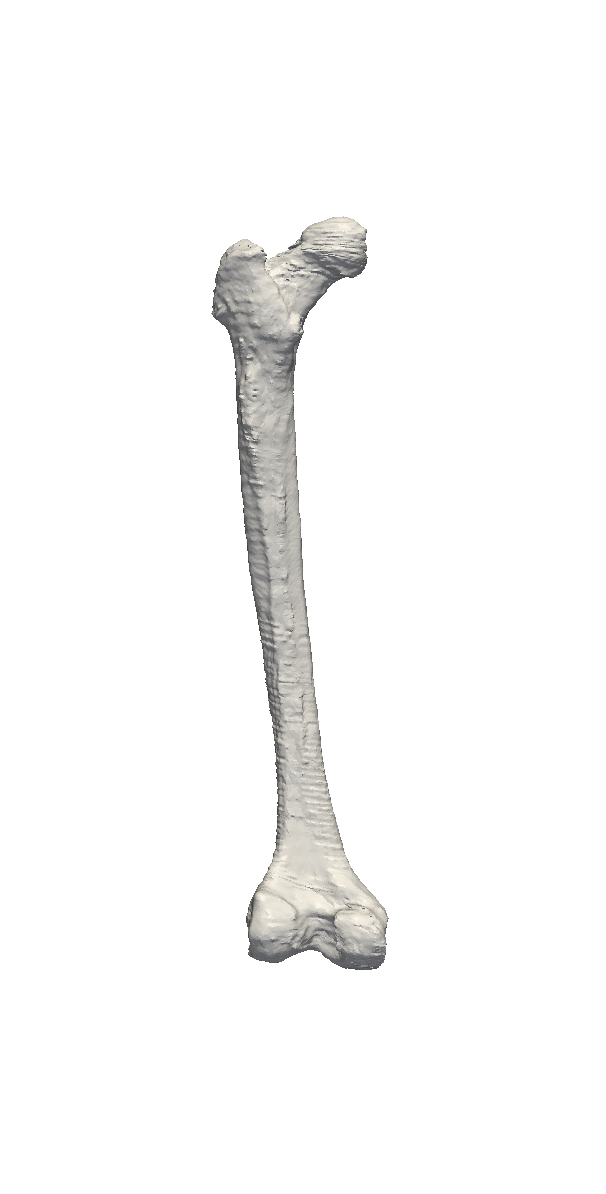
\includegraphics[width=0.3\textwidth]{pictures/femur-pc1m1.png}&
    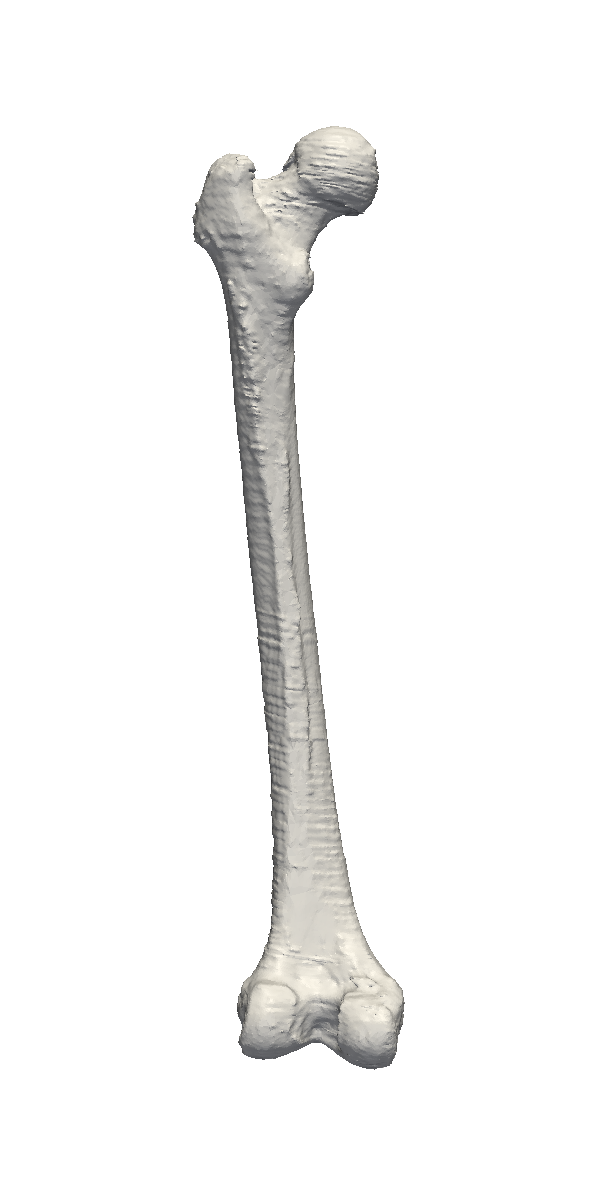
\includegraphics[width=0.3\textwidth]{pictures/femur-mean.png}& 
    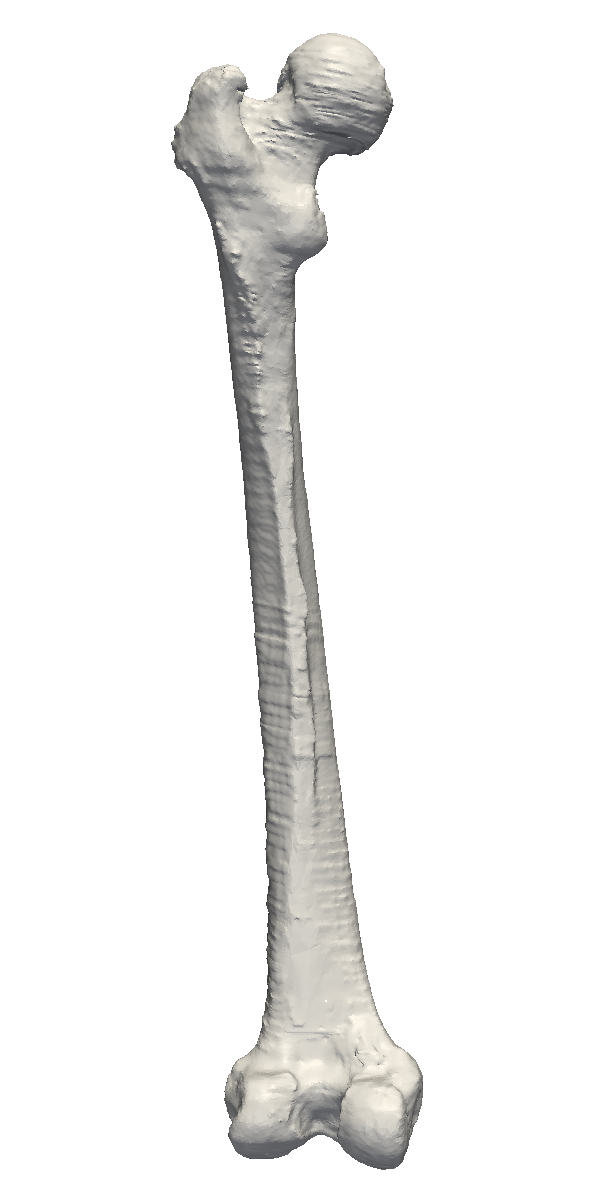
\includegraphics[width=0.3\textwidth]{pictures/femur-pc1p1.png}
    \\
    $-3 \sigma$ & mean & $+3 \sigma$
  \end{tabular}
  \itkcaption{The first mode of variation ($\pm 3$ standard deviations) for a shape model of the femur. 
    In this case the first variation mainly captures the size of the bone.}
    \label{fig:vispca}
\end{figure}


\subsection{Using statistical models as  a prior}
In many algorithms, statistical models are used as a shape prior. 
A common approach is to take an instance from an algorithm, and project it back into the 
shape space, to get an approximation of the given shape. In \Statismo, such a projection can be
obtained by computing the PCA coefficients for a given dataset and then restoring it using the 
\code{DrawSample} method:
\begin{verbatim}
vtkPolyData* dataset = someAlgorithm();
VectorType coeffs = model->ComputeCoefficientsForDataset(dataset);
vtkPolyData* projection = model->DrawSample(coeffs);
\end{verbatim}
Often, one simply regularizes an algorithm with the probability. For this purpose, \Statismo 
provides a method to compute a (log) probability of a given dataset. 
\begin{verbatim}
float logProbability = model->ComputeLogProbabilityForDataset(aDataset);
\end{verbatim}

\subsection{Cross validation}
An often neglected, but important task is the evaluation of
statistical models. One particular focus of interest is the
generalization ability of a model: the accuracy with which it is able to represent new instances of the object. 
This ability may be estimated through cross-validation studies. Cross-validation has also recently been employed
to derive confidence bounds quantifying the reliability of statistical model based prediction from partial observations \cite{blanc_estimating_2009,blanc_confidence_2012}. \Statismo provides convenience functionalities in order to facilitate such cross-validation studies. 

Cross-validation is done using the \code{DataManager}. 
After we have set up the \code{DataManager}, and populated it with the training data, we 
can obtain a list with cross validation folds. 
\begin{verbatim}
typedef DataManagerType::CrossValidationFoldListType CVFoldListType;
CVFoldListType cvFoldList = dataManager->GetCrossValidationFolds(4, true);
\end{verbatim}
Each entry of the \code{cvFoldList} contains a list of training samples and a list with the test samples. 
We iterate over all the folds and build for each fold a new model. A typical validation of the model would 
consist of computing an approximation error between the test sample, and its projection in the model. 
\begin{verbatim}
for (CVFoldListType::const_iterator it = cvFoldList.begin();
     it != cvFoldList.end();
     ++it)
{
    ModelBuilderType* builder = ModelBuilderType::Create();
    StatisticalModelType* model(builder->BuildNewModel(it->GetTrainingData(), 0.01));

    const SampleDataListType testSamplesList = it->GetTestingData();
    for (SampleDataListType::const_iterator it = testSamplesList.begin();
         it != testSamplesList.end()
         ++it)
    {
        vtkPolyData* testSample = (*it)->GetAsNewSample();
        vtkPolyData* projection = model->DrawSample(
                                         model->ComputeCoefficientsForDataset(dataset));
        /// here we could for example compute the approximation error between the 
        /// projection and the test sample - omitted

        testSample->Delete();
    }
    delete modelBuilder;
}

\end{verbatim}

\subsection{Model Fitting using the itk registration framework}\label{sec:model-fitting}
One of the most common applications of statistical models is to fit them to a patient dataset. 
In \Statismo this is done using the ITK registration framework. In the example 
we show how a shape model is fitted to an image using \code{itkPointSetToImageMetric}. 
In this example, we use the ITK wrapper of \Statismo, which allow us to use \Statismo objects as normal ITK objects.

We start with the usual type definitions. We use for this example a shape model, which has been 
built using the \code{itkMeshRepresenter}. 
\begin{verbatim}
typedef itk::Mesh<float, 3> MeshType;
typedef itk::ImageType<float, 3> ImageType
typedef itk::MeshRepresenter<float, 3> RepresenterType;
typedef itk::StatisticalShapeModelTransform<RepresenterType, double, 3> TransformType;
typedef itk::MeanSquaresPointSetToImageMetric<MeshType, ImageType> MetricType;
\end{verbatim}
The StatisticalShapeModelTransform is a class defined by \Statismo. It is a subclass of the \code{itk::Transform}
and can thus be directly used wherever an \code{itk::Transform} is expected. 

In the next step we load the model and obtain the reference mesh that was used to build the model via
the representer. This mesh is used by the \code{PointSetToImageMetric}, and determines the points on which the 
metric is evaluated. 
\begin{verbatim}
StatisticalModelType::Pointer model = StatisticalModelType::New();
model->Load(modelname);
MeshType::Pointer fixedPointSet  = model->GetRepresenter()->GetReference();
\end{verbatim}

The transform is set up by setting the statistical model, and initializing it to the identity transform. 
\begin{verbatim}
TransformType::Pointer transform = TransformType::New();
transform->SetStatisticalModel(model);
transform->SetIdentity();
\end{verbatim}

The registration is then set up in the usual way. We omit here the details.
\begin{verbatim}
MetricType::Pointer metric = MetricType::New()
...

RegistrationFilterType::Pointer registration = RegistrationFilterType::New();
registration->SetInitialTransformParameters(transform->GetParameters());
registration->SetTransform(   transform );
registration->SetFixedPointSet( fixedPointSet );
...
registration->Update()
\end{verbatim}

After a successful registration, the transform parameters correspond to the PCA coefficients in our model. 
To obtain the final mesh, we can obtain these coefficients from the transform using the method \code{GetCoefficients} 
and draw the corresponding sample from the model. 
\begin{verbatim}
MeshType::Pointer finalMesh = model->DrawSample(transform->GetCoefficients());
\end{verbatim}


\section{Adding more prior information: Constrained PCA models }
One goal of \Statismo is to allow the integration of  different algorithms for building statistical models.
Currently, \Statismo comes with three different methods to build statistical models (Cf. Figure~\ref{fig:class-diagram}). Besides the standard \code{PCAModelBuidler} that was used in all the examples presented so far, there is a \code{PartiallyFixedModelBuilder} \cite{luthi_probabilistic_2009} and a \code{ConditionalModelBuilder} \cite{blanc_conditional_2009}. Both model builders incorporate additional prior information into the model building and thus reduce the variability of the resulting model. The resulting models itself are standard PCA models that can be used and interpreted in exactly the same way as the models discussed so far. 
\subsection{Partially fixed models}
\begin{figure}[tbh]
  \begin{tabular}{ccc}
    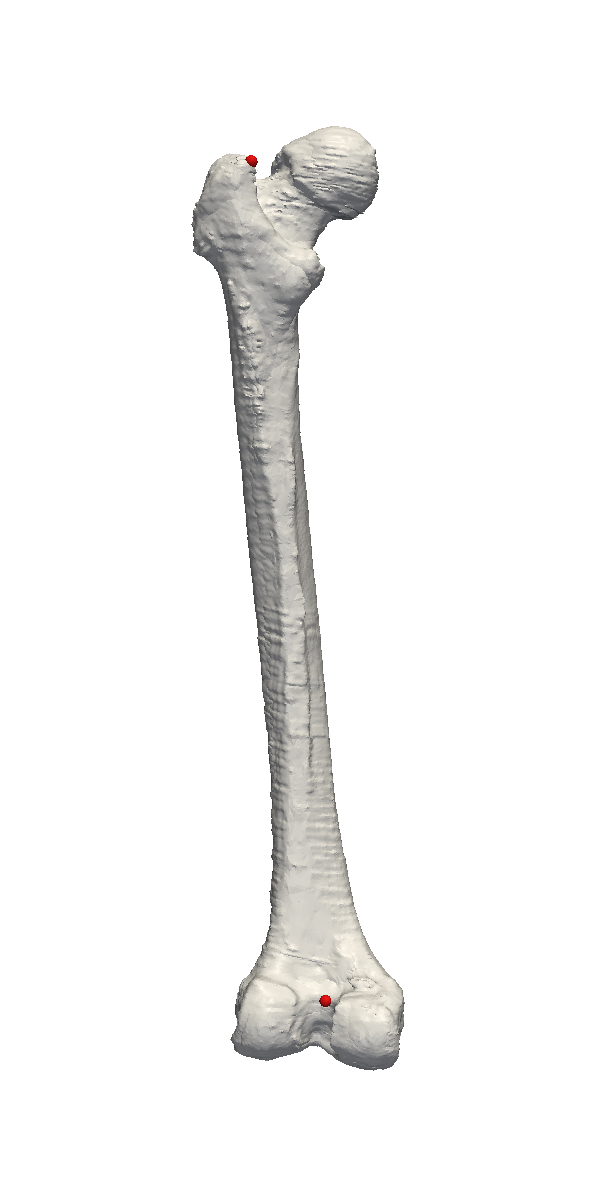
\includegraphics[width=0.3\textwidth]{pictures/femur-constrained-pc1m1.png}&
    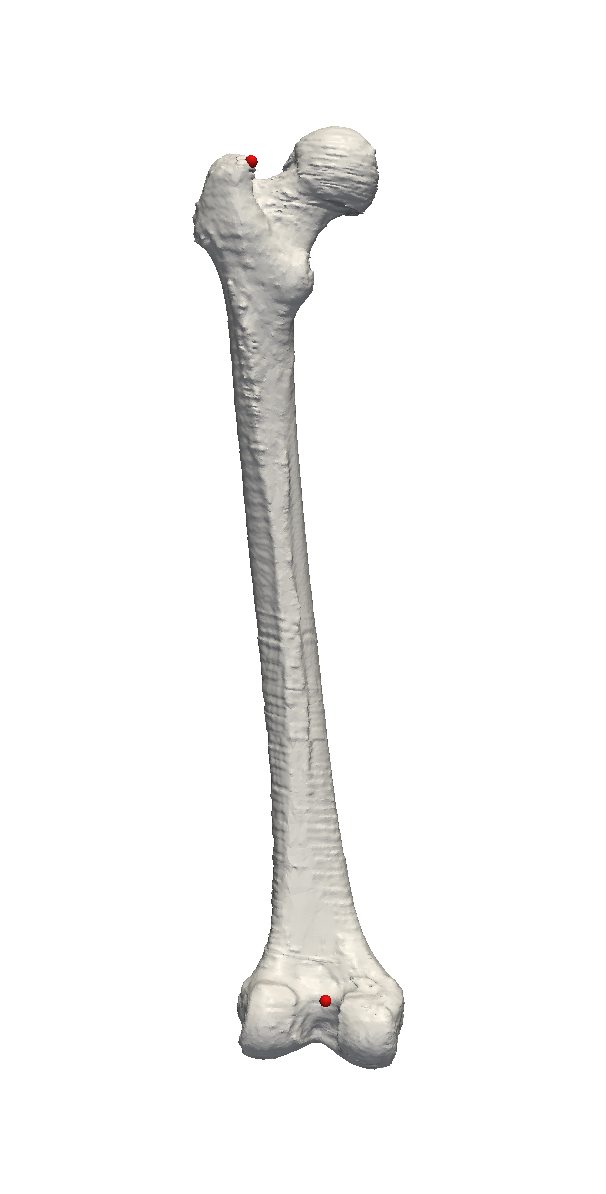
\includegraphics[width=0.3\textwidth]{pictures/femur-mean-lm.png}& 
    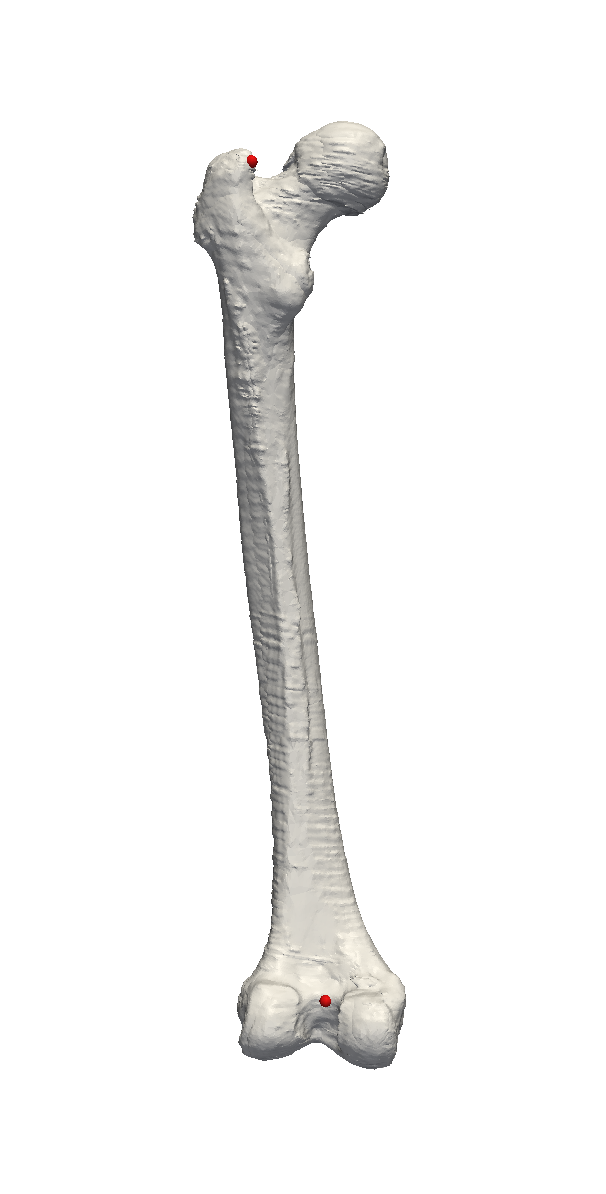
\includegraphics[width=0.3\textwidth]{pictures/femur-constrained-pc1p1.png}
    \\
    $-3 \sigma$ & mean & $+3 \sigma$
  \end{tabular}
  \itkcaption{A shape model of the femur, with two landmark points (in red) fixed. As the landmark points determine the size, 
  of the femur, the first component is not the size anymore, but shows mainly variations on the femoral head and the condyles. }
    \label{fig:constrained-model}
\end{figure}
Partially fixed models allow for introducing geometric constraints on
the model. This allows us to model the variability in a model, when we know the shape for a part of the model.
A typical application of this model is the reconstruction of a fractured or traumatized bone. 
Another scenario where these models are useful is in model fitting. 
Consider the shape model fitting example from Section~\ref{sec:model-fitting}. Assume
that we know for some points of the model the corresponding points on the target image. 
Using the \code{PartiallyFixedModelBuilder}, we can
incorporate these constraints into the model building, to obtain a
model that represents only shapes that match the target points.  The
following (incomplete) code illustrates how such models can be built.
\begin{verbatim}
// ... usual type definitions - omitted
typedef PartiallyFixedModelBuilder<RepresenterType> PartiallyFixedModelBuilderType;

PartiallyFixedModelBuilderType*  pfmb = PartiallyFixedModelBuilderType::Create();

// ... Read model and target landmarks, omitted

StatisticalModelType::PointValueListType constraints;
for (unsigned i = 0; i < numLandmarks; i++) { 
   StatisticalModelType::PointValuePairType cnstr(modelLandmarks[i], targetLandmarks[i]);
   constraints.push_back(cnstr);
}
StatisticalModelType* constraintModel = 
   pfmb->BuildNewModel(dataManager->GetSampleData(), constraints);
\end{verbatim}
Figure~\ref{fig:constrained-model} shows the first main variation for
the same shape model as in Figure~\ref{fig:vispca}, but this time with
2 points (in red) fixed. We see that the landmark point remain fixed
in the first main variation.  By using this constrained model for model fitting, we can thus guarantee that
the landmark points are matched, without having to change our fitting
algorithm. An additional advantage is that the search space becomes
smaller, and thus the optimization problem easier.  For more details
on the theoretical background and the applications of these models, we
refer to the papers \cite{luthi_probabilistic_2009,luthi_using_2011}.

\subsection{Conditional Models}
The second algorithm for model building, which we refer to as the
\emph{ConditionalModelBuilder} for constrained model is used when
there are additional surrogate information about the data available.
The underlying idea is to exploit such information to generate a
statistical model of the object variability given prescribed
constraints. \Statismo handles both continuous and categorical types
of surrogates.  To achieve this, the potential useful surrogate
variables have to be associated to the training samples.

A special \code{DataManagerWithSurrogates} is provided for this
purpose. When creating such a data manager, a file describing the
number and types of variables is passed as an argument.  The class has
a special method to add datasets together with the associated
surrogate data: \code{AddDatasetWithSurrogates(dataset, surrogateFilename)}
(the exact format of these input files is described in the internal documentation).

In order to learn a conditional model, the user then specifies which
of surrogate variables are used for conditioning, and specifies the
corresponding values against which the model should be conditioned by
filling a structure of type \code{ConditionalModelBuilder<RepresenterType>::CondVariableValueVectorType}.

In this implementation, only the training samples which respect the
requested categories are selected.  Continuous variables are used to
learn a conditional distribution of the variability, using a simple
assumption of joint multivariate normality. Practically speaking, an
unconditional statistical model is first learned using the
PCAModelBuilder class using the selected training sample. The PCA
coefficients of each of these training samples are computed, and
pooled with the requested continuous surrogates. Assuming a joint
multivariate gaussian distribution for this set of variables, the
conditional distribution of the model coefficient given the prescribed
constraints is derived. The assumption of multivariate normality then
allows to reformulate this conditional model in the reduced space back
into the original high dimensional space. Therefore, the obtained
conditional model is expressed in the exact same mathematical
formulation as standard PCA models.  The implementation is currently
limited to cases where the number of retained training samples (after
selection based on categories) is larger than the number of original
PCA coefficients retained plus the number of continuous surrogate
variables used as conditions.

More details, and possible extension to more complex distributions
models can be found in \cite{blanc_conditional_2009}.

\section{Conclusion}
In this paper we have presented \Statismo, which is a framework for
PCA based statistical models.  \Statismo implements a high level view
on PCA models by interpreting these models as normal distribution over
the modeled objects. The underlying low level vectorial representation
of the object is never exposed to the user.  The conversion between
the data representation by the user, and the vectorial representation
used by \Statismo is done by special Representer classes, which are
defined for each data representation. This allows \Statismo to ensure
that the same discretization and normalization steps are applied when
using the model, as those that were used during model building.  A
statistical model in \Statismo thus always have a well defined
interpretation and semantics.  This, together with the fact that
\Statismo writes all its information into a single, portable HDF5
file, makes the exchange of statistical models built with \Statismo
easy. To use the model, the user only needs to have access to the same Representer that was used to build the model. 

\Statismo comes with ready made Representer classes for the most important object representations used in VTK and ITK. 
Currently all these representers require that the data is already in correspondence. It is, however, easily possible to 
write representers that also establish correspondence, and thus to cover the full model creation pipeline with \Statismo.
By writing custom representers, it becomes also possible to use \Statismo with other toolkits than ITK or VTK. 

Statismo also makes it easy to integrate new methods for building models. Our hope is, that the number of different representers
and model builders will grow and thus \Statismo will become a more and more powerful toolkit for building a large variety of differnet 
models.



\appendix

\section{Appendix}


\subsection{The file format}
\Statismo uses the platform independent HDF5 \cite{hdf5} to save the
statistical models. The HDF5 file contains all the information that is
needed to use the model from an application as well as information
about the data and parameters used to create the model.  HDF5 provides
a hierarchical, file-system like data organization. 
For \Statismo, we have organized the data into  3 main groups:
\begin{description}
  \item [Model] Contains the vectors and matrices that define the model, i.e.\ the \code{mean}, the \code{pcaBasis}, the \code{pcaVariance} as well 
    as the \code{noiseVariance} assumed in the model. 
  \item [Modelinfo] Holds the metadata for the model. The metadata
    consists of the \code{buildtime} of the model, the \code{scores} (the
    PCA coefficients of the original example data), a section using 
    \code{builderInfo} that contains all the parameters of the specific model builder used to build the model, as well as a section \code{dataInfo} that contains the URI's of the datasets that have been used to build the model. 
  \item [Representer]
    This group is used to store all the information that is needed by the representer. 
 \end{description}
 The data stored in the HDF5 file can eihter be explored using the API provided by \Statismo (Cf. the class \code{StatisticalModel}), or directly 
 from one of the many software packages that support HDF5, such as e.g.\ Matlab \cite{matlab}, R \cite{R} or Pytables \cite{pytables}.

\subsection{Currently available Representers}
\Statismo comes with several Representer classes for building various types of statistical models, using VTK and ITK. 
Currently, all the representers requires that the input datasets are discretized in the same way and in correspondence.

In the following we briefly describe the different Representers:
\begin{description}
\item[TrivialVectorialRepresenter] This is the most basic representers. It can be used to build statistical models in the case where the input is already available in a vector representation. 
\item[vtkPolyDataRepresenters] Used to build shape models from VTK, in case where the data is represented as VTK Polydata. This representer 
  performs a Procrustes alignment \cite{horn_closed-form_1987} of the datasets before the model is built. 
\item[vtkStructuredPointsRepresenter] This representer is used to
  build image (appearance-) and deformation models from data that is
  represented as vtkStructuredPoints. 
\item[itkMeshRepresenter] This representer is used to build shape
  models from itk Meshes.  In contrast to the vtkPolyDataRepresenter,
  no alignment is performed.
\item[itkImageRepresenter] Used to build 2D and 3D image (appearance-) models from itk images. 
\item[itkVectorImageRepresenter] Used to build 2D and 3D deformation models from itk displacement fields. 
\item[itkVectorImageLMAlignRepresenter] This representer is similar to the itkVectorImageRepresenter. 
  In addition, the user can provide a number of landmark points. the input displacement fields are evaluated
  at these landmark points, to obtain a set of corresponding points. From these points, a rigid transformation is computed, 
  which is used to resample the displacement fields. 

\end{description}

\subsection*{Acknowledgements}
This work has been supported by the CO-ME/NCCR research network of
the Swiss National Science Foundation. The femur data has been made available by the Virtual Skeleton Database (VSD) project\footnote{http://www.virtualskeleton.ch}. We also would like to thank Arnauld Gelas for helpful comments regarding this
submission. 



%%%%%%%%%%%%%%%%%%%%%%%%%%%%%%%%%%%%%%%%%
%
%  Insert the bibliography using BibTeX
%
%%%%%%%%%%%%%%%%%%%%%%%%%%%%%%%%%%%%%%%%%

\bibliographystyle{plain}
\bibliography{InsightJournal}


\end{document}

